%% muonDetectionSystem.tex
%%

%% ==============
\chapter{Muon detection system}
\label{ch:The muon detection system}
%% ============== 
  The need for low background rates at the main detector requires for a good knowledge of background sources. Despite magnetic reflection and wire electrodes, cosmic ray and particularly cosmic muon induced background may be an issue for the KATRIN experiment. To gather and asess muon related data, scintillator modules have been installed at both the monitor spectrometer and the main spectrometer. While the monitor spectrometer is equipped with only two rather small modules, at the larger main spectrometer, 8 modules have been installed at different positions enabling the user to cover different regions of the vessel (see figure \ref{fig:modulesMainSpec}). This freedom is enlarged by installing the detection system on three independently movable trolleys.
  The modules have been connected to the DAQ one trolley per card, meaning modules one and two connect to card three, modules 3 through 5 to card six and modules 6 through 8 to card nine (\ref{tab:connectionsModulesCards})
  \begin{table}
  	\centering
  	\begin{tabular}{| l | c c | c c | c c | c c |}
  	\hline
  		Module	& 1A	& 1B	& 2A	& 2B	& 3A	& 3B	& 4A	& 4B 	\\
  		Card	& 3	& 3	& 3	& 3	& 6	& 6	& 6	& 6	\\
  		Channel	& 0	& 14	& 3	& 7	& 0	& 14	& 3	& 7	\\
  		\hline \hline
  		Module	&5A	& 5B	& 6A	& 6B	& 7A	& 7B	& 8A	& 8B	\\
  		Card	& 6	& 6	& 8	& 8	& 8	& 8	& 8	& 8	\\
  		Channel	& 9	& 23	& 0	& 14	& 3	& 7	& 9	& 23	\\
  		\hline
  	\end{tabular}
  	\caption[Channel assignment]{Assignment of module sides to cards and channels}
  	\label{tab:connectionsModulesCards}
  \end{table}
  \begin{figure}
  	\centering
  	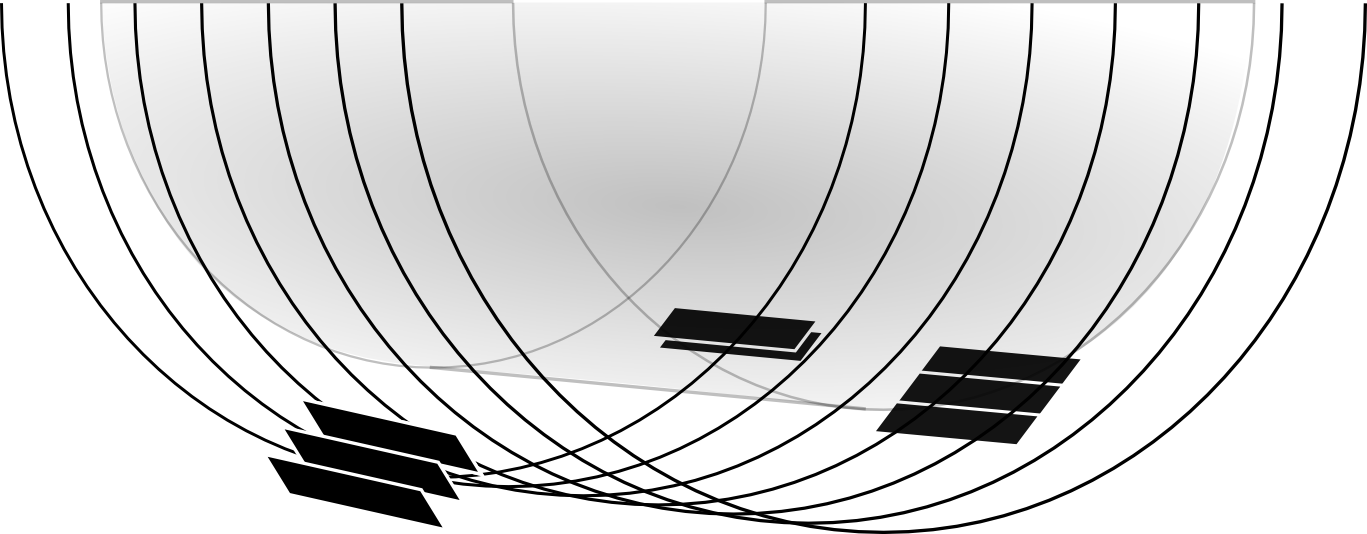
\includegraphics[width = 0.9 \textwidth]{graphics/muonModules/mainSpec/panelsMainSpec.png}
  	\caption[Module locations]{An overview over the module positions in relation to the main spectrometer and its LFCS system. }
  \end{figure}

  All connections from modules to DAQ are made of coaxial cabling of equal length. This ensures comparable timestamps which are assigned only after the analogue signals arrive at the DAQ. High voltage is provided by two supplies, one on the east and one on the west side of the main hall.
  All devices of the muon detection system are connected to two multiplugs that are both overcurrent protected and feature mains filters. These multiplugs have been modified \ref{fig:multiplug} to connect to a ground other than the outlet's. To ensure a common potential for all of the devices and the surrounding appliances this connection was made to the trough below the main vessel.
  \begin{table}
  \centering
  	\begin{tabular}{|c|c|c|c|c|c|}
  	\hline
  		V0 & I0 & I1 & V1 & Ramp Up & Ramp Down\\
  		\hline
  		\SI{1.5}{\kilo\volt} or \SI{1.6}{\kilo\volt} & \SI{2000}{\milli\ampere} & & & \SI{50}{\volt} & \SI{100}{\volt}\\
  		\hline
  	\end{tabular}
  	\caption[High voltage settings]{High voltage settings as used for the muon modules. Modules XX and XX are set to \SI{1.6}{\kilo\volt}.}
  	\label{tab:HVSettings}
  \end{table}

  \begin{figure}
  \centering
  
  	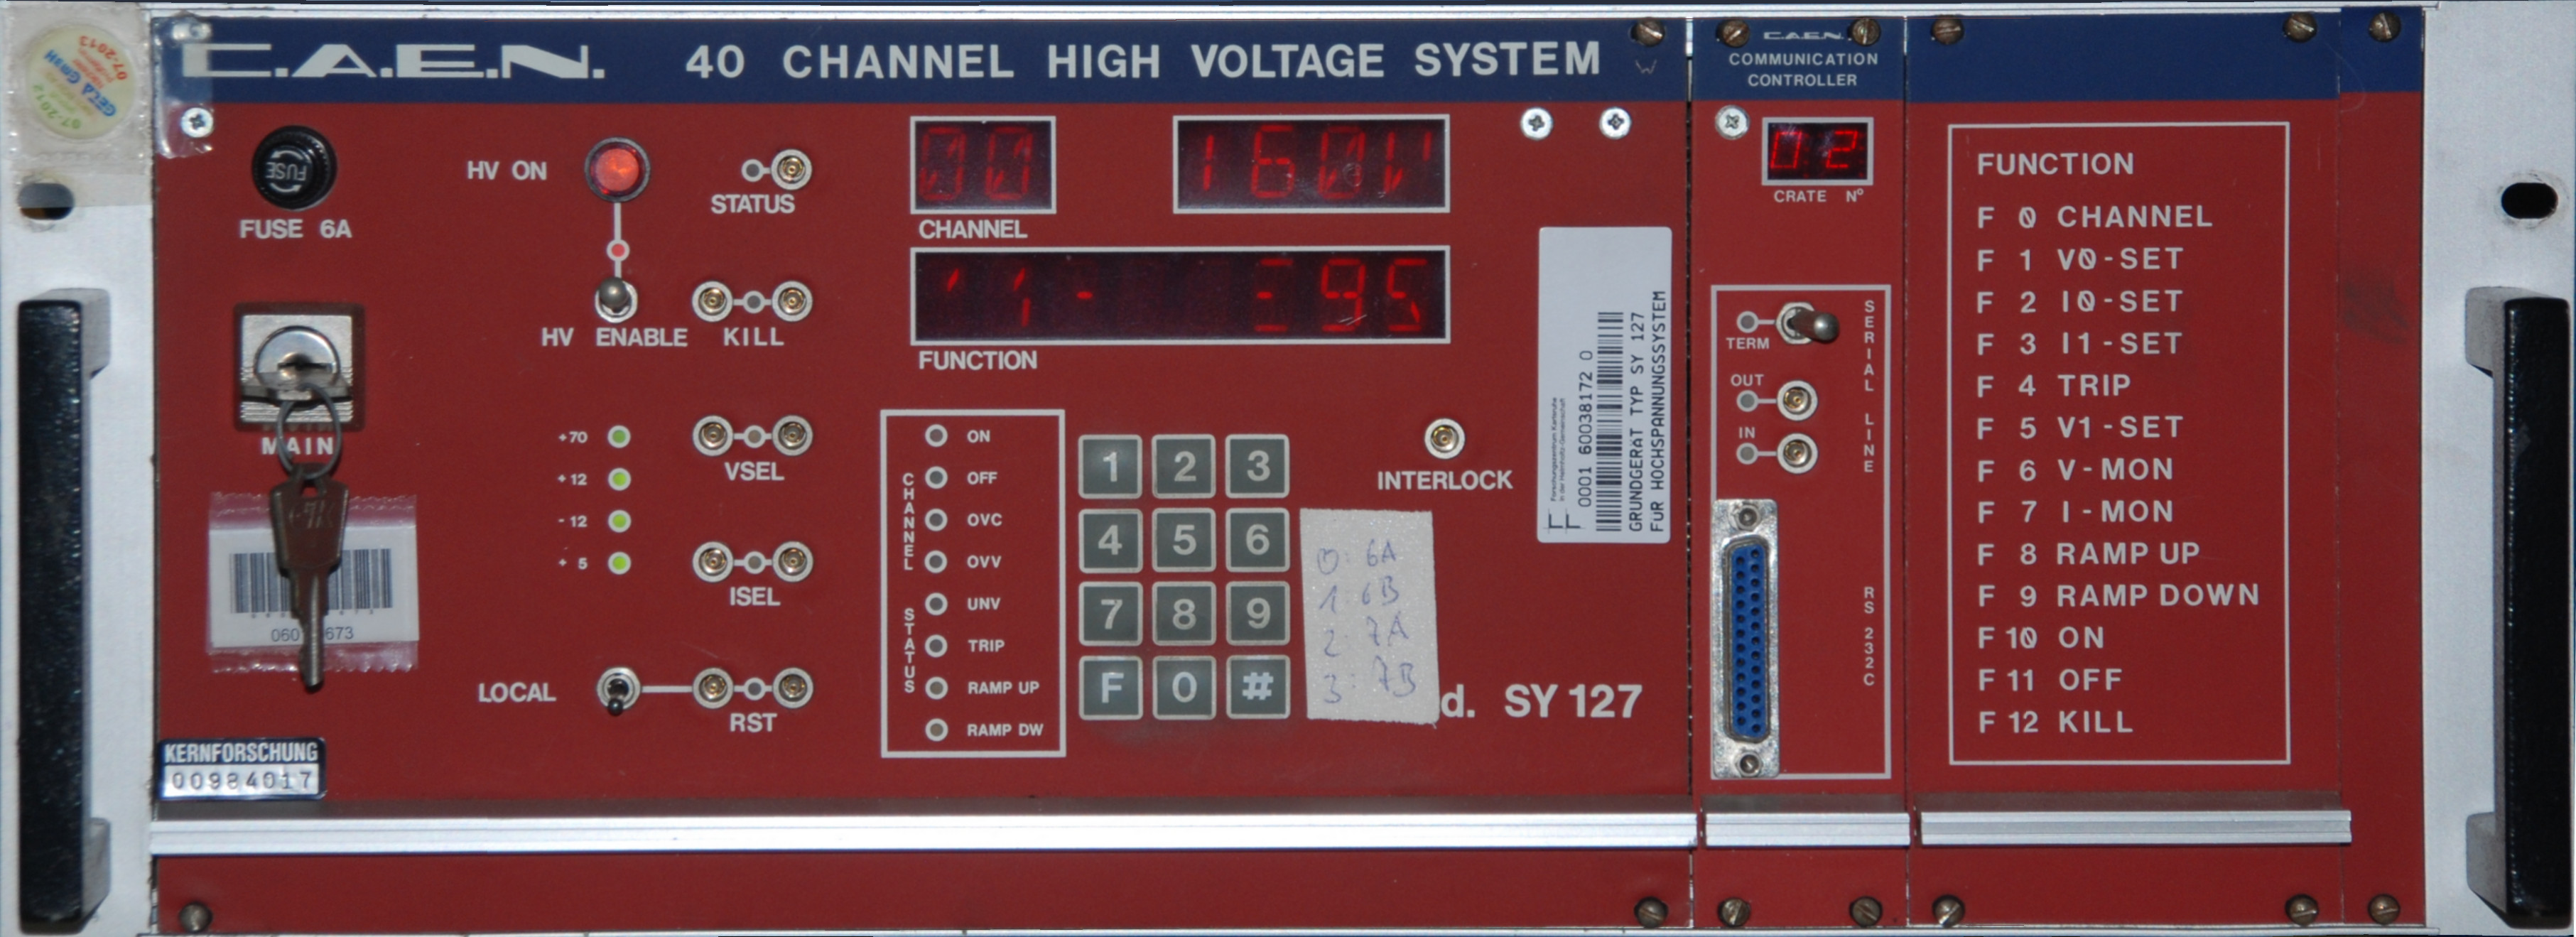
\includegraphics[width = \textwidth]{graphics/muonModules/mainSpec/HV.jpg}
  \caption[High voltage supplies]{A photograph of one of the two high voltage supplies used to power the muon modules photomultipliers. On the right side, the codes for setup are visible, see table \ref{tab:HVSettings} for the settings used.}
  \label{fig:multiplug}
  \end{figure}
\todo{insert photograph of multiplug}


%% DAQ.tex
%%

%% ==============
\section{Data aquisition crate}
\label{ch:DAQ}
%% ==============
The Data acquisition crate, short DAQ, is the central part of event recording and by that the interface between hardware muon modules and software based ORCA machine. It was developed for the Pierre-Auger-Observatory in the first place, but was then distributed to many different experiments due to its large flexibility and the There are two types of DAQs used in KATRIN: the standard one and the mini DAQ used at the monitor spectrometer. The latter features only 4 FLT plus one SLT slot which is sufficient for the monitor spectrometer, but not for the main detector. Here, the larger model with up to  It features first and second level trigger cards in version \SI{4}{} that are described in detail in the following sections \ref{ch:DAQ:sec:FLTs} and \ref{ch:DAQ:sec:SLTs}. The Linux based system runs from an external hard drive connected to the second level trigger card via USB. Here, a screen and keyboard can be connected for network setup, then, access via secure shell is possible. The DAQ can be connected to and controlled by the ORCA software \ref{ch:The muon detection system}. 

  \begin{figure}
  \centering
  
  	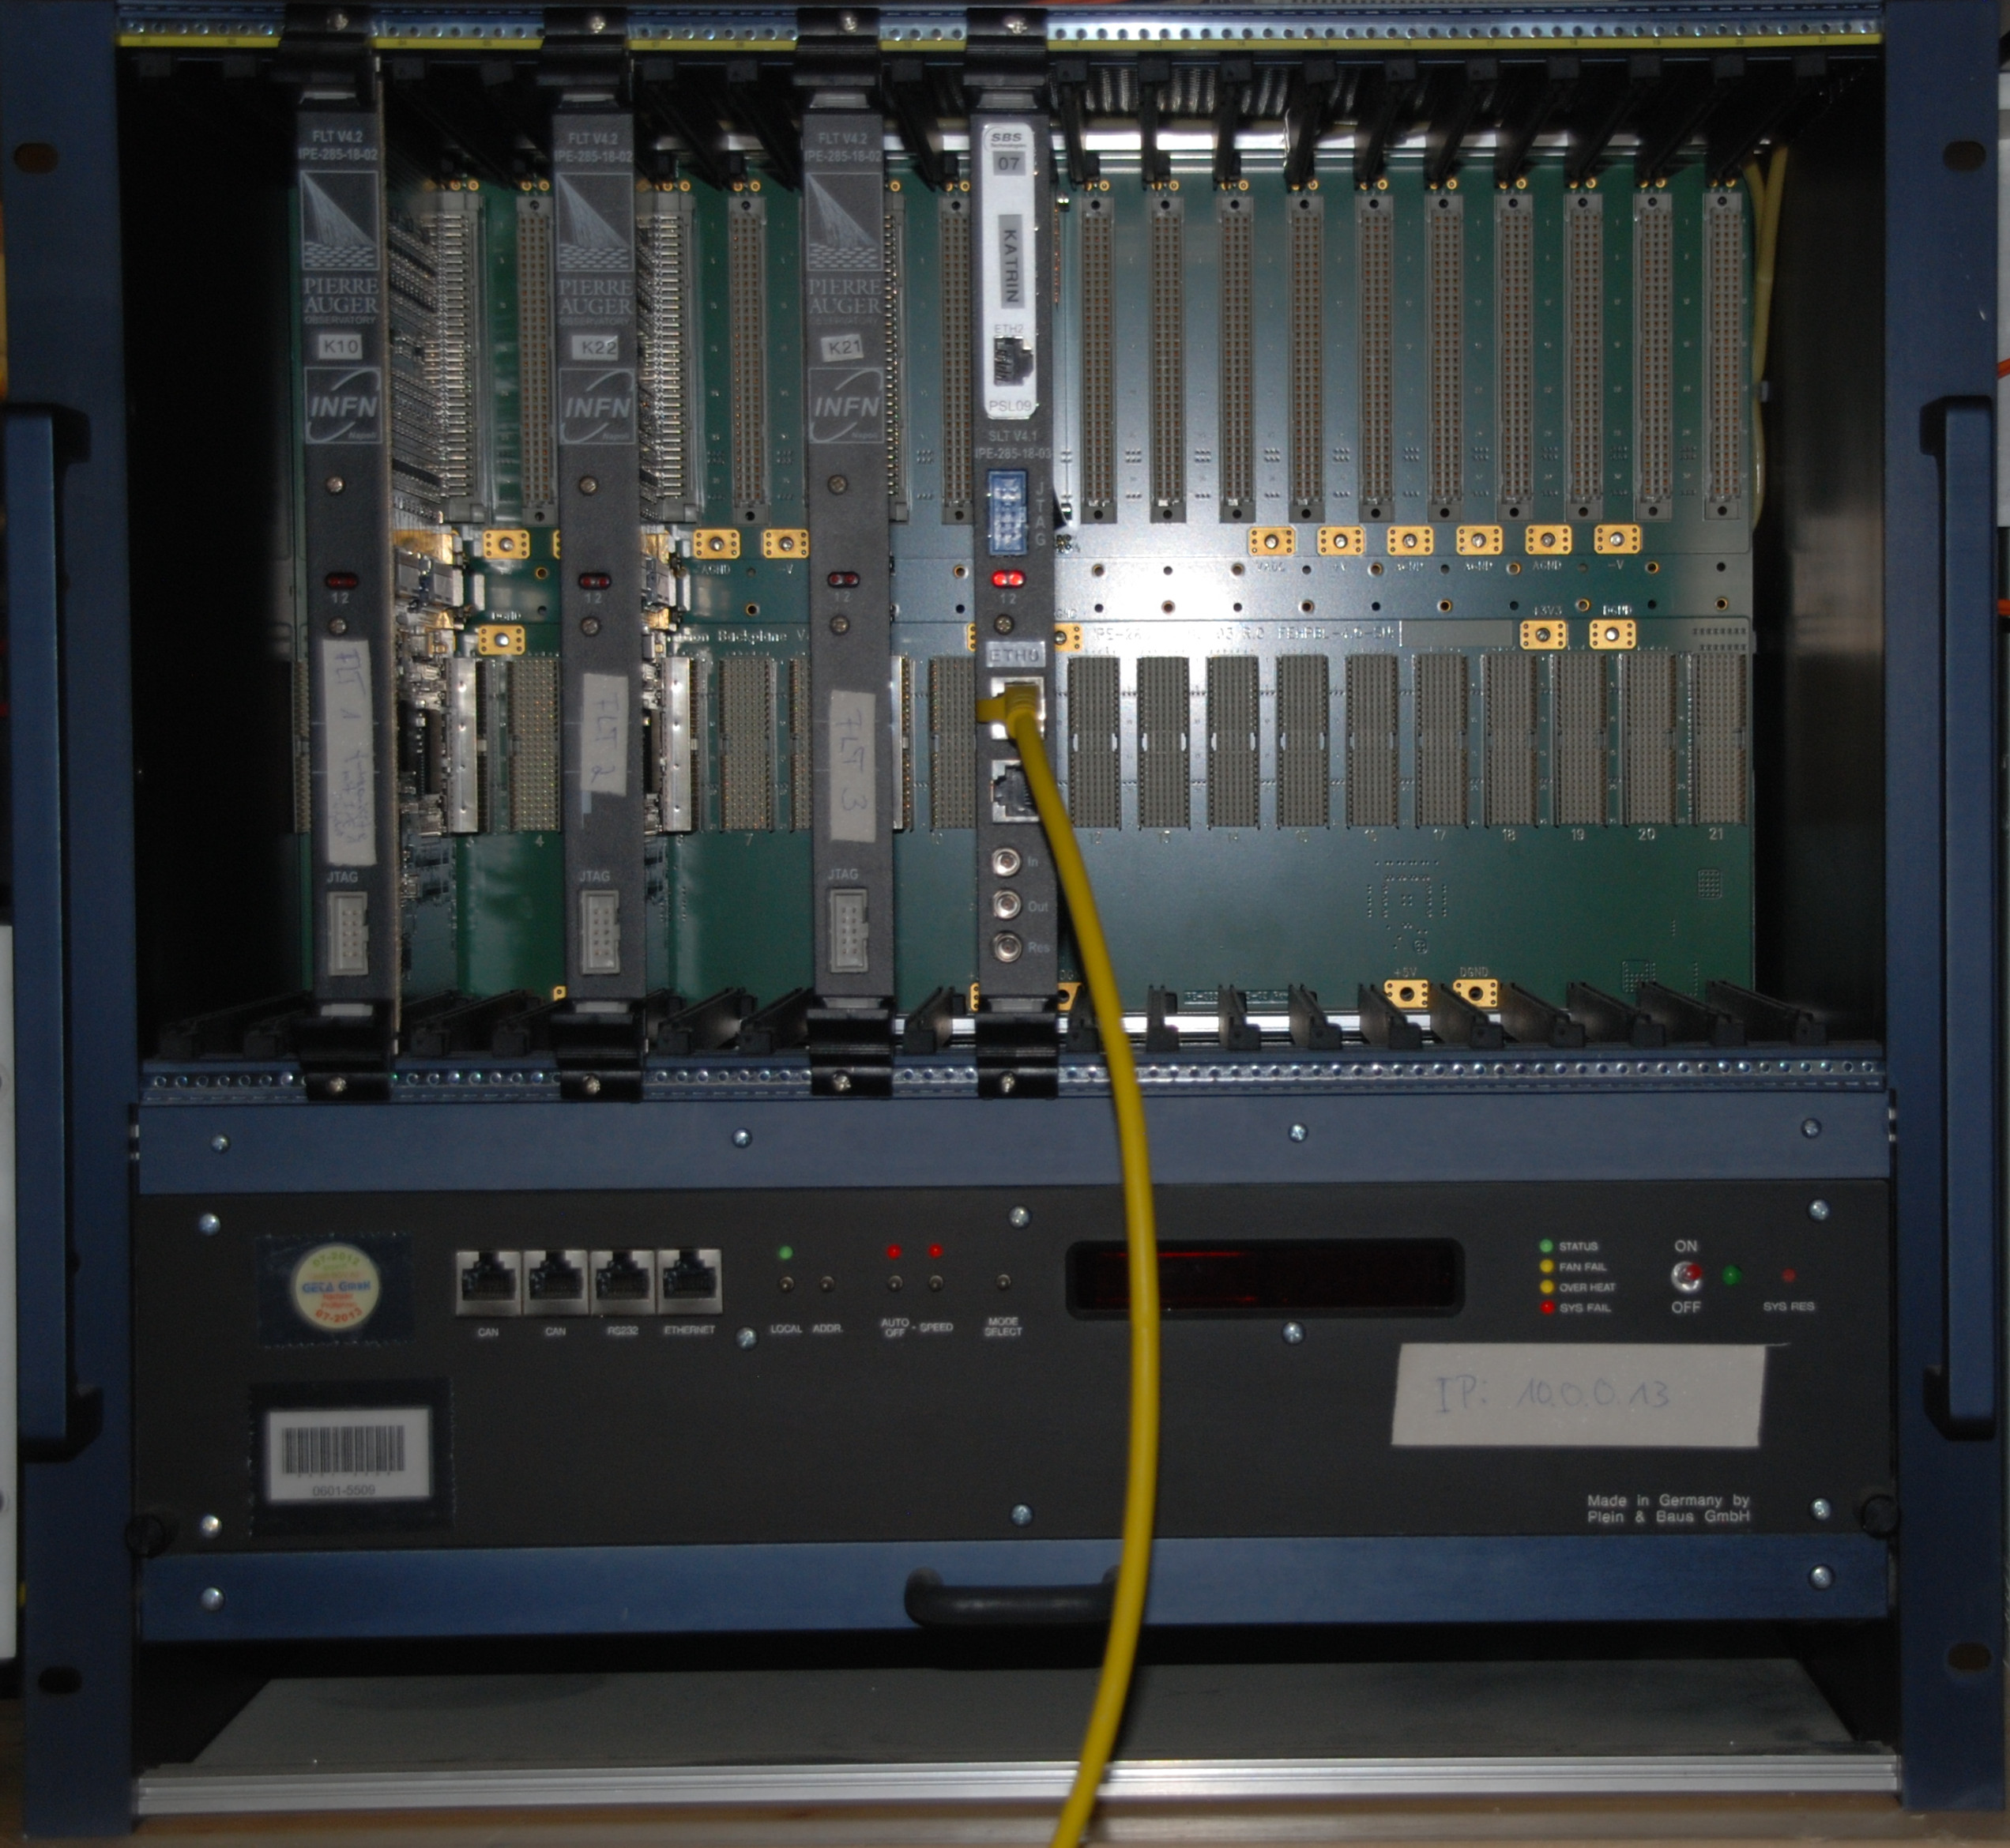
\includegraphics[width = 0.7 \textwidth]{graphics/muonModules/mainSpec/DAQ.jpg}
  \caption[Data acquisition crate]{A image of the data acquisition crate's front panel. From left tor right, the three FLT cards and the SLT card with its ethernet connection are visible.}
  \label{fig:DAQ}
  \end{figure}

  %% ===========================
  \subsection{First level trigger cards}
  \label{ch:DAQ:sec:FLTs}
  %% ===========================
  The FLT cards directly receive the signal output of the photomultiplier tubes via coaxial cabling. They then do first parts of data analysis to reduce data flow to the ORCA machine. In this case, only events with occur simultaneously on both sides of any module are passed on. This reduces the rate from \todo{look up non veto rate} to around \SI{250}{\hertz}. The FLT cards are made up of a large main card and a smaller connector card entered at the back side. Every card has 28\todo{28?} channels. These are sectioned into three groups if the card is operated in veto mode. then, every group consist of one sum channel that can be read out in coincidence with any other or multiple other channels from the group (see figure \ref{fig:DAQ:FLTFront}). In case of the muon modules, 1-fold coincidence is used; one side of each module is the sum channel, the other an arbitrary channel in the respective group.
  
  \begin{figure}
	  %\includegraphics[width=0.5\textwidth]{graphics/DAQ/FLTBack.}
	  \caption[FLT back panel card]{FLT back panel card with channel numbering scheme. Readout groups are 0,1,2,3,4,5,6,7 with 14 as the sum channel,}
	  \label{fig:DAQ:FLTFront}
  \end{figure}
  \begin{figure}
	  %\includegraphics[width=0.5\textwidth]{graphics/DAQ/FLTFront.}
	  \caption[FLT back panel card]{FLT back panel card with channel numbering scheme. Readout groups are 0,1,2,3,4,5,6,7 with 14 as the sum channel,}
	  \label{fig:DAQ:FLTBack}
  \end{figure}
  \todo{channel numbers}\ref{fig:DAQ:FLTFront}
  %% ===========================
  \subsection{Second level triger cards}
  \label{ch:DAQ:sec:SLTs}
  %% ===========================
  Only one second level trigger card is installed on each DAQ. all the Signals from the FLT cards are stacked here and passed on to the the ORCA machine. Networking runs directly through the SLT card. Other connections, such as USB, a display port, and also the CAT 5 connectors for synchronization to a clock can be attached to the back panel card.

  %% OrcaControl.tex
%%

  %% ==============
  \section{Orca control}
  \label{ch:OrcaControl}
  %% ==============
  The ORCA software (Object-oriented Real-time Control and Acquisition) \cite{How09} is the central software for data acquisition. It is able to control lots of different devices via various kinds of interfaces with Ethernet connections being the most common.

    %% ===========================
    \subsection{Software Gains and Thresholds}
    \label{ch:OrcaControl:sec:SoftwareGainsThresholds}
    %% ===========================
    All data registered by the DAQ is amplified and cut off at certain, software set values. Theses can be entered for every channel of every card separately. Gains can vary from \SI{0}{} to \SI{4095}{} (\SI{12}{\bit}), thresholds can be set to any value up to the maximum bin used. Depending on the filter settings, ore more precisely with rising shaping length, bin values will be shifted  towards higher absolute values \ref{ch:Analysis:sec:Finding the best filter settings}.
    Scripting of the values is possible and reasonable for large numbers of readout channels such as at the FPD.
    
	\begin{figure}
		\raggedright
% 		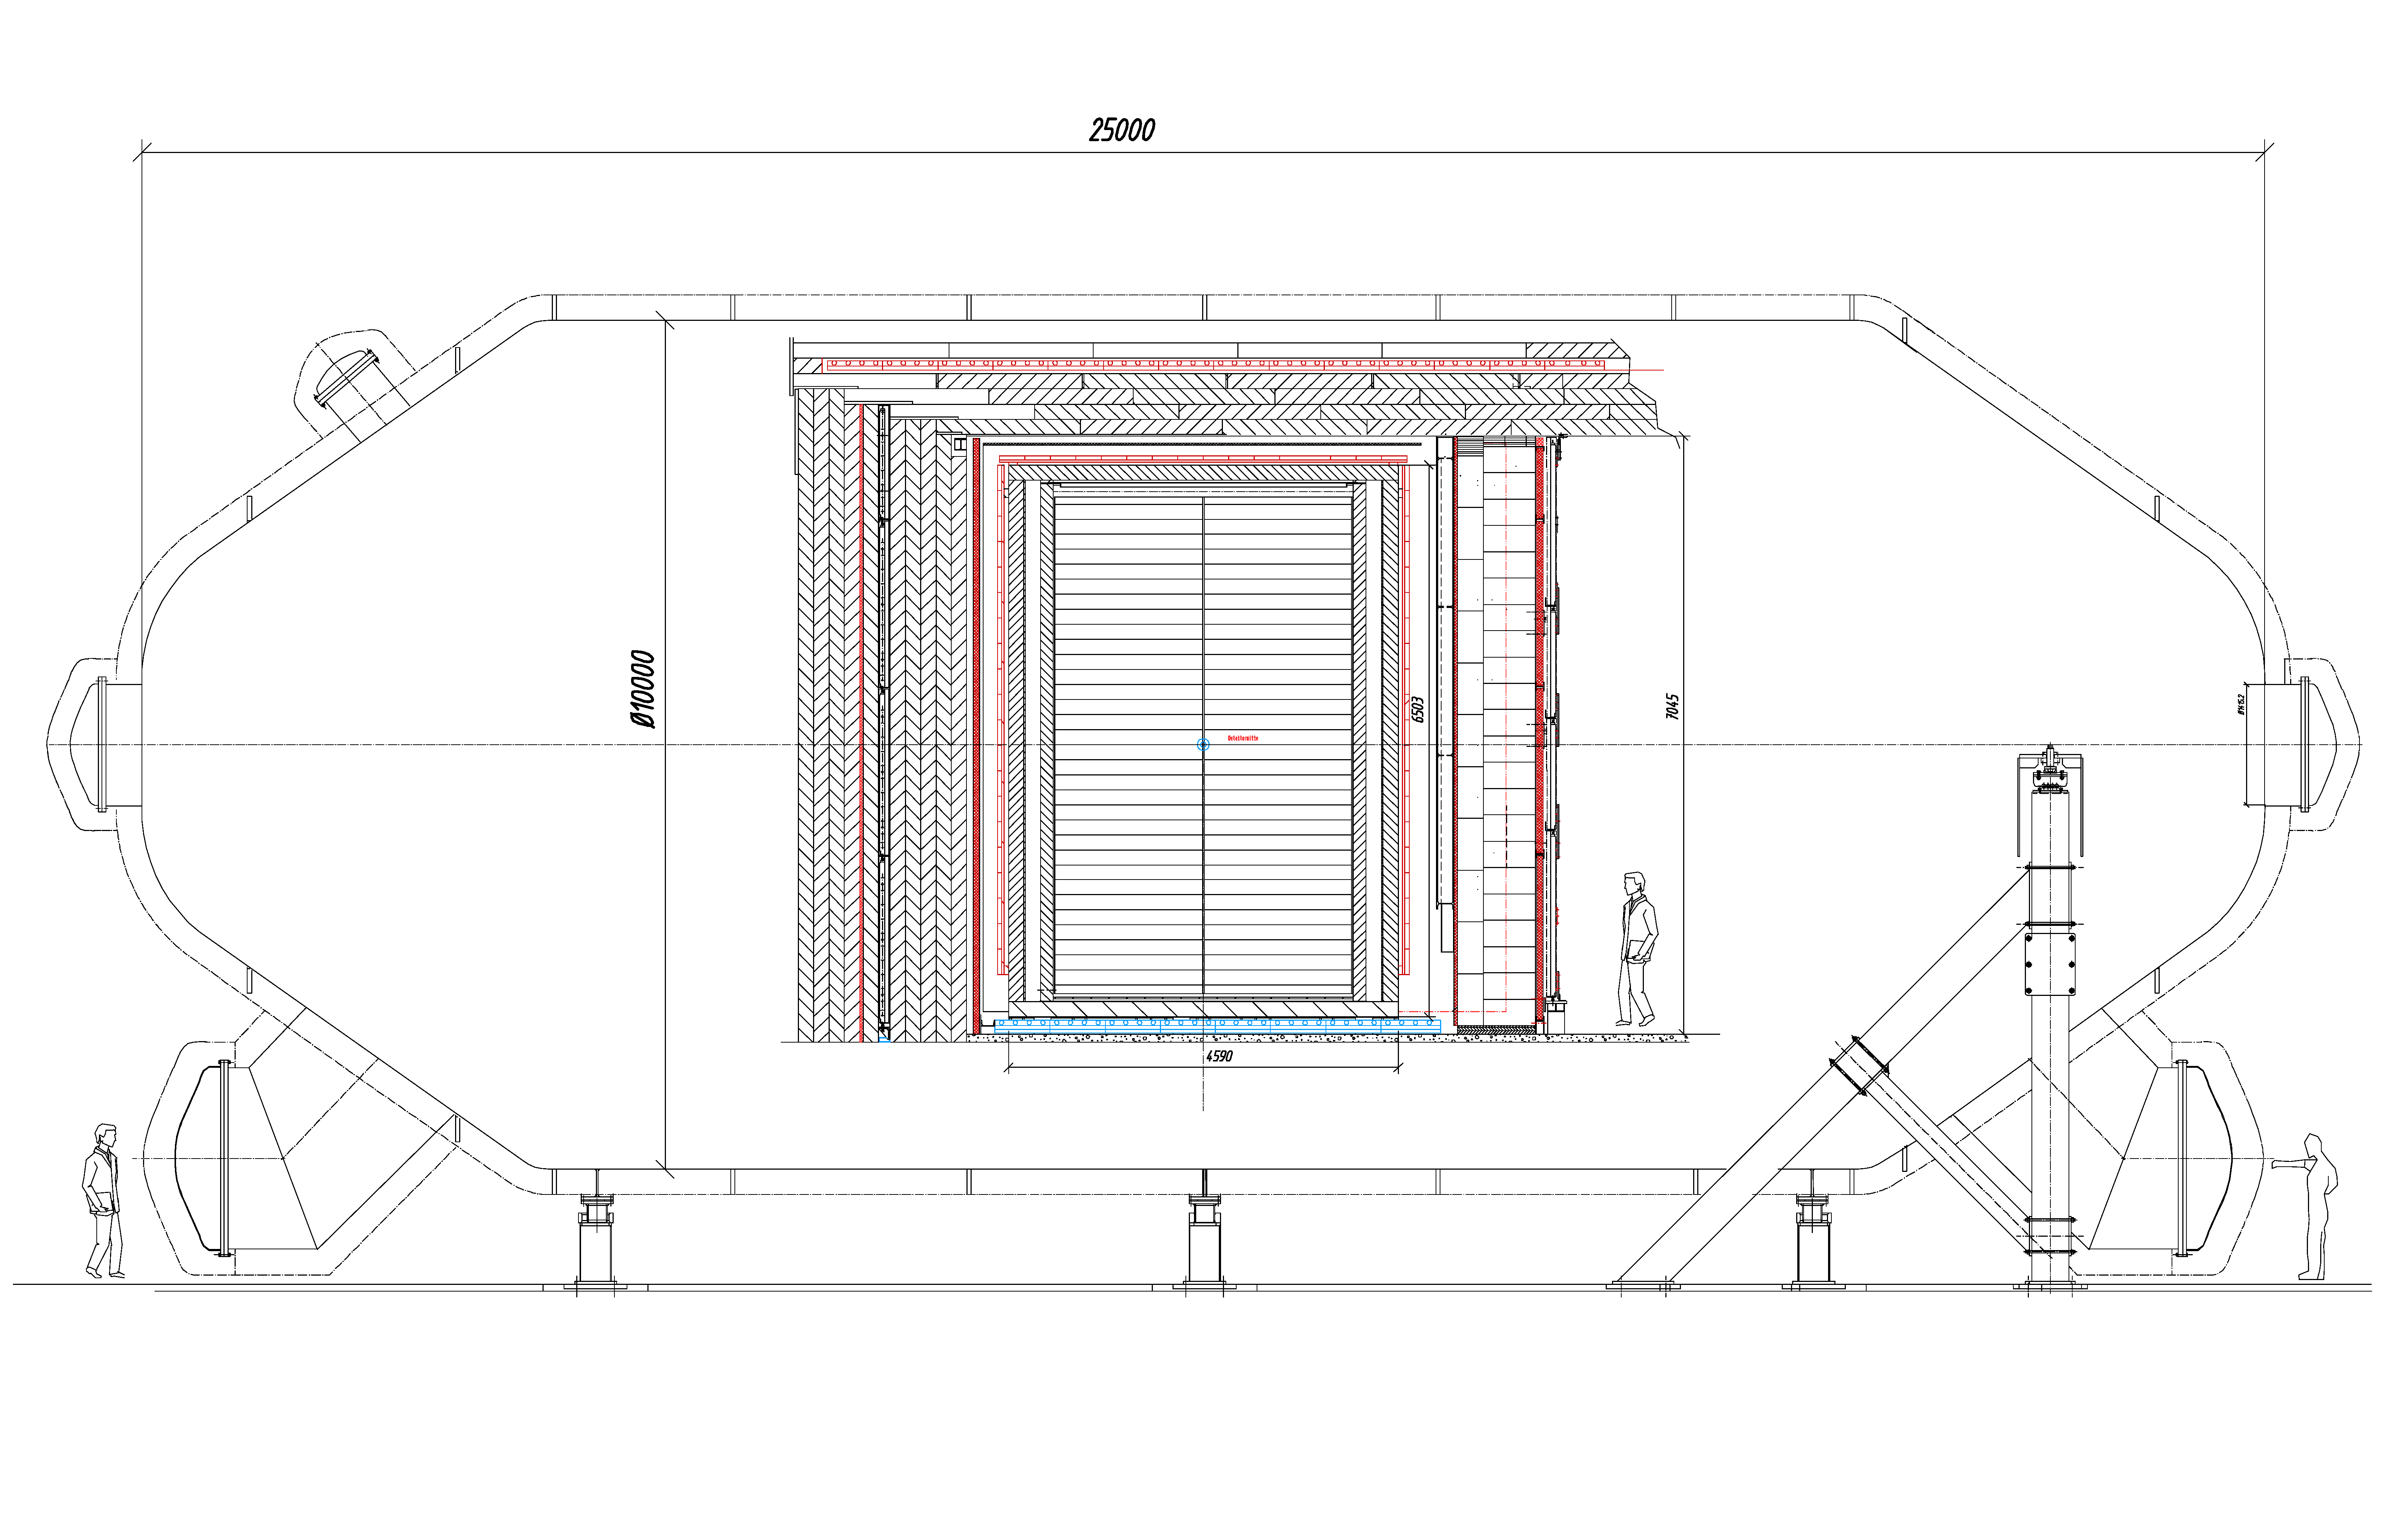
\includegraphics[width = 0.4 \textwidth]{graphics/muonModules/mainSpec}
		\caption[Multiplug grounding]{Added extension of the earthing contact to connect to any ground needed}
		\label{fig:multiplug}
	\end{figure}
    
    %% ===========================
    \subsection{Run control}
    \label{ch:OrcaControl:sec:RunControl}
    %% ===========================
    Runs are the basic element of data storage, every time data is recorded, a run is created. Inside every run can be a number of subruns (at least there is one) that will in turn contain data classes such as KaLi::KLVetoEvents, the most used event class in case of the muon modules. Runs and Subruns are started and stopped via the "Start Run", "Stop Run", "Start SubRun" and "Stop SubRun" buttons. While, from Run control, Runs can be set to end after a certain timespan and even repeat, Subruns can only be used on the go. This is different if scripting is utilised. \ref{ch:OrcaControl:sec:Scripting}.
    
    %% ===========================
    \subsection{Scripting}
    \label{ch:OrcaControl:sec:Scripting}
    %% ===========================
    Scripts are useful for repetitive tasks or such that require short interaction only at certain points in time. One example for scripting is the ramping of LFCS coils that has been used to check the rate dependence on the LFCS currents. In that case, the script sends the values to be set to the ZEUS server, which passes them on to the \todo{company name} boxes which in turn set the desired values at the power supplies. As this was supposed to be a stability measurement, every LFCS setting was kept constant for half an hour after which the script changed the currents. Scripting makes it possible to take these \SI{5}{\hour} runs without human interaction making it much more comfortable \ref{fig:ORCA:script}. Of course, much more sophisticated tasks can be handled through scripts as well.
    
    %% ===========================
    \subsection{File handling}
    \label{ch:OrcaControl:sec:FileHandling}
    %% ===========================
    All runs created are first saved to the local disc of the iMac machine as ORCA specific .orca files. Sorting in folders for year and month can be applied to quickly find what you are looking for. They are then uploaded to servers of the IPE via cronjobs, a feature of the Linux based MacOS. The crontab is set to upload only files from "/home/../data/" \todo{add dirs} - the folders in the data storage object should be set to that \ref{fig:ORCA:dataStorage}. Scripts on the servers convert the files to the .root format. Using the ROOT based KaLi software, the user can then access and analyse \ref{ch:Analysis software:sec:Data structure} this data from anywhere he has Internet access. 
    
    \begin{figure}
    	%\includegraphics[width = 0.5\textwidth]{graphics/ORCA/dataStorage}
    	\caption[ORCA data object]{Data storage obect in ORCA. Marked is the dropdown for setting paths for data, logs and ...}
    	\label{fig:ORCA:dataStorage}
    \end{figure}

    
    %% ===========================
    \subsection{Orca Fit}
    \label{ch:OrcaControl:sec:OrcaFit}
    %% ===========================
    The Orca Fit function uses external servers to fit data aquired by the DAQ in user defined ways. Besides linear or gaussian fits, landau fitting can be used. This way, the user can receive an impression of the goodnes of the data via $R^2$ values.
  
  
  %% ===========================
  \section{Scintillator modules}
  \label{ch:The muon detection system:sec:Scintillator modules}
  %% ===========================
  The central part of the detection system are the eight scintillator modules. They are made of the synthetic material BC-412 which is utilized in applications requiring large area coverage \cite{scintillatorManual}. These have previously been used at  \todo{From Where?}. Every scintillator cuboid is read out by two sets of four photomultiplier tubes. Photons arriving at the short ends of the module are guided to the photomultiplier tubes via non-scintillating material which, away from that, exhibits similar optical properties. All other sides of the scintillator are covered in reflective foil to push detection efficiency to the maximum.
  \begin{figure}
    \centering
    
\includegraphics[width = 0.9\textwidth]{graphics/dummy.eps}	
  \end{figure}
  Of the eight photomultiplier tubes per scintillator module installed, 4 are read out via one FLT channel. The background of low energy events can be reduced significantly by recording only events occuring on both sides of the module at once. Only coincident signals should be recorded by the DAQ, though, on some occasions, quite a lot of single side signals occur. To account for those, every dataset is first analysed by a search algorithm (\ref{ch:Analysis software:sec:Search algorithms:subsec: Incremental Search}) to filter them.
  

  
  
  %% ===========================
  \section{Photomultipliers}
  \label{ch:The muon detection system:sec:Photomultipliers}
  %% ===========================
  Photomultipliers work on two fundamental principles: photoemission and secondary emission.
  Each Photomultiplier tube is made up of a layer of bialkali metal where photons from scintillation ionize the layers' atoms leaving electrons with their initial energy less the ionization energy.
  $$E_{e^-} = E_{phot} - E_{ion}$$
  The electron is then accellerated and guided by the electric field from dynode to dynode (see figure \ref{fig:PMT}), cascading to more and more electrons, as each electron's energy rises by $e\cdot U_{acc}$ between each pair of dynodes.
  \begin{figure}
  	\centering
  	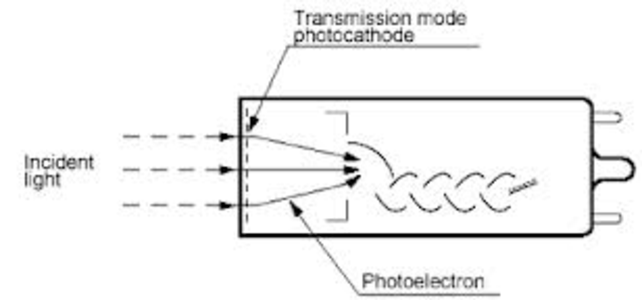
\includegraphics[width = 0.5 \textwidth]{graphics/setup/PMT.pdf}
  	\caption[Photomultiplier tube]{Schematic view of a photomultiplier tube with incident photons and photo-electrons emerging. Note the nested dynode structure for cascading purposes.}
  	\label{fig:PMT}
  \end{figure}

  
  
  %% ===========================
  \section{Gains, Thresholds and Acceleration Voltages}
  \label{ch:The muon detection system:sec:Gains, Thresholds and Acceleration Voltages}
  %% ===========================

	To achieve the best possible event detection, the photomultipliers' acceleration voltages as well as the software gains and thresholds in Orca had to be adjusted.
	The focus here was to obtain landau peaks with equal heigt and width, as the rates throughout the modules can be considered equal over large time intervals compared to the inverse rate.
	At first, the acceleration voltages were kept low to limit the signal peaks' heigts to aroud \SI{2}{\volt}. Carefully setting the mentioned parameters, one achieved the following, well alligned curves. A problem remaining at the time though was that the electronic noise set in pretty close to the peak position, only slightly shifted to lower energies. This meant that thresholds hat to be set close to the peak bin as well, loosing low energy events in the process, observable in figure \ref{fig:allPeaksBefore}. This showed in rates of around \SI{150}{\hertz} that did not compare too well to literature values. The high energy region though was well fittable with landau distributions.\\
	\todo{mv co}
	\begin{figure}
		\centering
		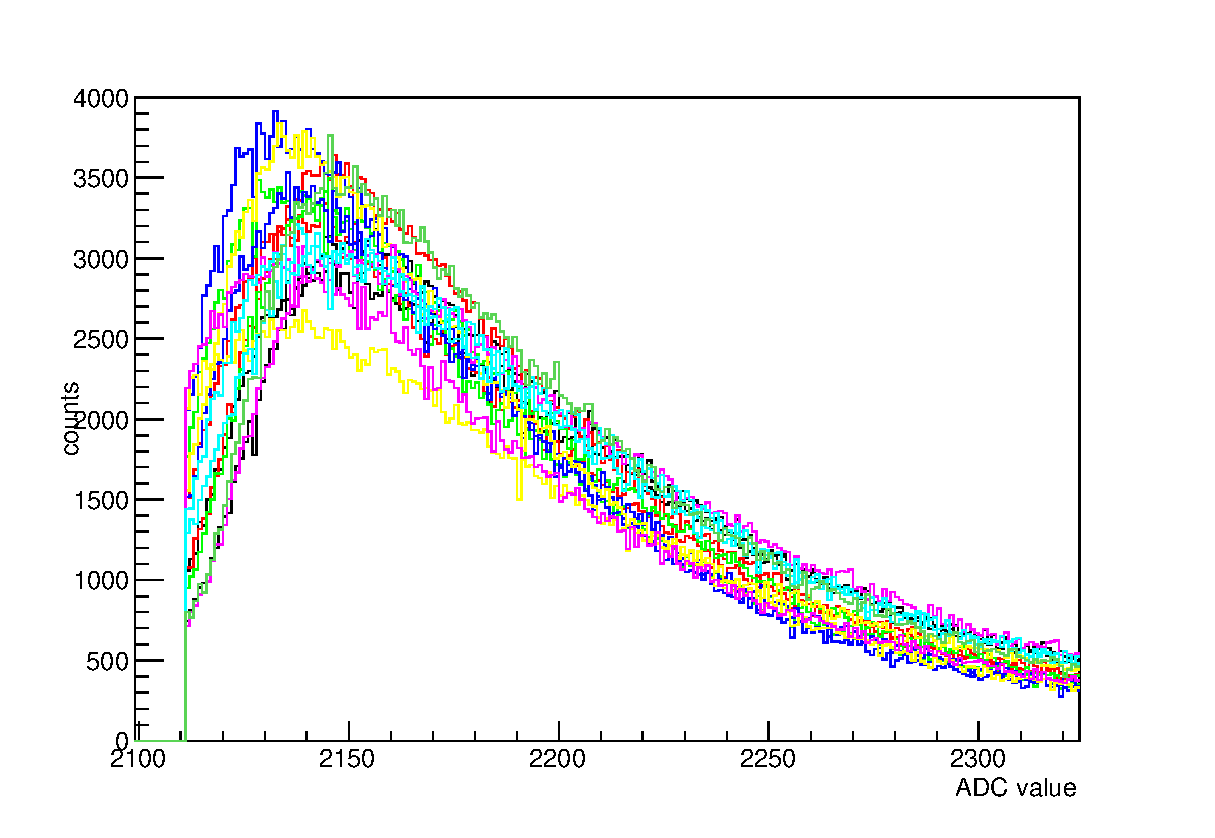
\includegraphics[width = 0.9 \textwidth]{graphics/setup/LandauPeaksRun660_old.eps}
		\caption[Landau peak \SI{1200}{\volt} acceleration voltage]{The landau peak at acceleration voltages around \SI{1200}{\volt}. All channels show similar width and height. Note that the threshols had to be set pretty close to the peak position as noise was a huge issue under the conditions.}
		\label{fig:allPeaksBefore}
	\end{figure}\\
	Later in the comissioning process, it got clear from the handbooks that the photomultiplier tubes had to be operated at accelleration voltages of \SI{1.5}{\kilo\volt} and above. To keep the singnals' height as small as possible, most of the tubes were limited to this minimal voltage, wheras the sides \todo{which ones} were set to \SI{1.6}{\kilo\volt} over showing lower rates than the others. Following this procedure, the tubes seemed much more stable and comparable, as all the gains and thresholds could now be set to the same values of \todo{enter values} and respectively, while still showing aligned peak positions \ref{fig:allPeaksAfter}. This is a huge advance to before when gains varied by a factor of up to almost four as it reduces potential non-linearities in amplification. Also, gains are left at lower values to begin with, leaving a larger part of the al in all amplification to the photomultiplier tubes known for their linear behaviour and relatively low noise.
  
	\begin{figure}
		\centering
		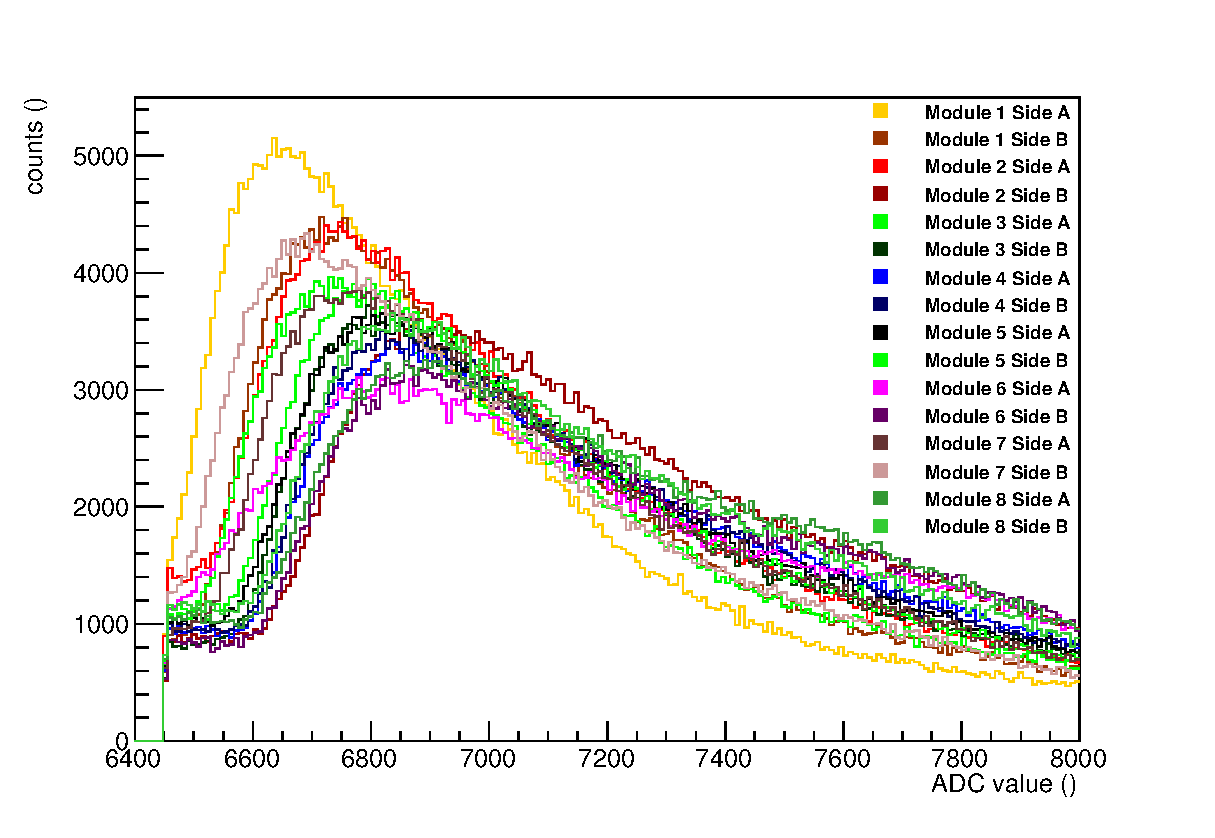
\includegraphics[width = 0.9 \textwidth]{graphics/setup/LandauPeaksRun1097_new.eps}
		\caption[Landau peak \SI{1500}{\volt} acceleration voltage]{Landau peaks after raising acceleration voltages to \SI{1.5}{\kilo\volt} or else \SI{1.6}{\kilo\volt}. Note that this pattern was achieved solely by raising two module's side's acceleration voltages to \SI{1.6}{\kilo\volt} leaving gains and thresholds at the same low level for all channels. }
		\label{fig:allPeaksAfter}
	\end{figure}



